\documentclass{standalone}
\usepackage{tikz}
\usetikzlibrary{patterns, angles}
\usepackage{circuitikz}

\begin{document}
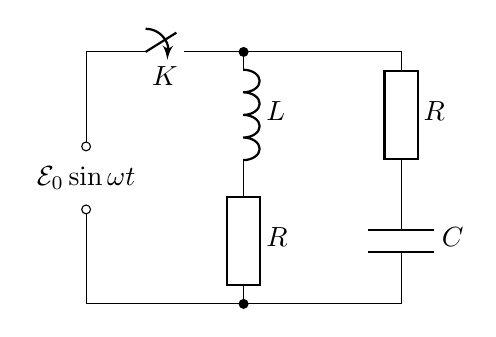
\begin{tikzpicture}[european]
	\draw (0,0) to [switch,-*] (2,0) to [american inductor, l=$L$] (2, -1.6) to [R,l=$R$,-*] (2,-3.2) -- (0,-3.2) to [short,-o] (0,-2.0) (0,-1.2) to [short,o-] (0,0)  (2,0) -- (4,0) to [R,l=$R$] (4,-1.6) to[capacitor,l=$C$] (4, -3.2) -- (2,-3.2);
	\node at (0,-1.6) {$\mathcal{E}_0 \sin \omega t$};
	\node at (1,-0.3) {$K$};
\end{tikzpicture}
\end{document}